
\documentclass[12pt,a4paper]{article}

\usepackage[utf8]{inputenc}
\usepackage{lmodern}
\usepackage[T1]{fontenc}
% paysage
% \usepackage[landscape]{geometry}
\usepackage{lscape}
\usepackage{graphicx}
% \graphicspath{ {images/} }

% headers footers
\usepackage{fancyhdr}
\pagestyle{fancy}

% référencer la dernière page
\usepackage{lastpage}

% pdf
\usepackage{pdfpages}

% math
\usepackage{amssymb}

\usepackage{multicol}
\usepackage{url}

\usepackage{multido}
\usepackage[utf8]{inputenc}
% \usepackage{lmodern}
\usepackage[T1]{fontenc}

\usepackage[sfdefault]{AlegreyaSans} %% Option 'black' gives heavier bold face
%% The 'sfdefault' option to make the base font sans serif
% \renewcommand*\oldstylenums[1]{{\AlegreyaSansOsF #1}}

\usepackage{breqn}
\usepackage{multicol}

% \usepackage{pstricks,pst-plot,pst-node}
% \usepackage{pstricks-add}
\usepackage{pst-circ}
\usepackage{pst-magneticfield}
\usepackage{pst-electricfield}
\usepackage{graphicx}
\usepackage{amsmath,amsfonts,amssymb}
\usepackage{titlesec} 
\usepackage{float}
\usepackage{textcomp}
\usepackage{amssymb}
\usepackage[toc,page]{appendix}
\usepackage{listings} 

\lstset{language=Matlab}
\usepackage{lipsum}
\usepackage{enumerate}


%Numerotation par section des équations
\usepackage{amsmath}

\usepackage{tabularx}
\usepackage{longtable}

%------------------------------inclue les références
% \usepackage[nottoc, notlof, notlot]{tocbibind}
%\usepackage{biblatex}
% \usepackage{csquotes}

%\usepackage{etoolbox}
% \patchcmd{\chapter}{\thispagestyle{plain}}{\thispagestyle{fancy}}{}{}
\title{
	\Huge\textsc{Engine output power}
}
\author{Mohamed Thebti} 

\begin{document}
	% retrait de la première ligne d'un paragraphe
	\setlength{\parindent}{0mm}
	
	\fancyhead[R]{\slshape \leftmark}
	\fancyhead[L]{\slshape Engine output power}
	%\fancyhead[LE,RO]{\slshape \rightmark}
	% \fancyhead[LO,RE]{\slshape \leftmark}
	
	% \fancyfoot[C]{Travail de Master}
	\fancyfoot[L]{\slshape Mohamed Thebti}
	\fancyfoot[C]{}
	\fancyfoot[R]{\thepage}
	
	\maketitle
	\newpage
	
	\tableofcontents
	
	\newpage
	
	
	\section{Introduction}
	
	The main objective of this report is compute the thermodynamics cycle of a combustion engine and the corresponding output power generated. 
	Secondary objective : torque profile $T(RPM)$, efficiency $\eta$, fuel consumption profile according to the engine RPM.
	
	% 
\includegraphics[scale=.2]{oxford-2021-01.jpg}
	
	
	\section{Engine power}
	
	The total engine power of the sum of the power produced from each piston. 
	As each piston has the combustion stroke at different time (crankshaft angle), the piston power must be computed according to crankshaft angle and firing order of the engine. 
	Step 1 : compute power produced by 1 piston
	Step 2 : shift the power profile for the piston according to its number and firing order.
	Example : I4 -> 1-3-2-4 : 
	$alpha_1$ = $alpha_crankshaft$\\
	$alpha_2$ = $alpha_crankshaft + 360$\\
	$alpha_3$ = $alpha_crankshaft + 180$\\
	$alpha_4$ = $alpha_crankshaft + 540$\\
	\subsubsection{Combustion chamber pressure}
	Gasoline engine : .... cycle
	
	Diesel engine : Diesel cycle
	
	
	
	\begin{enumerate}
		\item compute pressure and power with thermodynamic cycle
	Study the combustion to estimate its efficiency:
	\begin{equation*}
		\eta_{combustion}=\frac{q_{out}}{q_{in}} \tag{1}
	\end{equation*}	
	$q$ : energy $[J / kg]$
	
	The results is per $[\mathrm{kg}] \rightarrow \mathrm{J} / \mathrm{kg}, W / \mathrm{kg}, \ldots$\\
	
	\subsection{Engine dimensions}
	choose the size of the combustion chamber, the piston head diameter, the connecting rod length, 
		\item choose the mass flow $\dot{m}$, the displacement, and size of combustion chamber. -> we can compute power in $W$ and pressure in $Pa$\\
	$V_{\min }$ is the volume when the piston is at TDC\\
	$V_{\text {max }}$ is the volume when the piston is at BDC\\
	
	\begin{equation}
		V_{max} = V_min + disp \cdot S_{piston} = V_{min} + disp \cdot \pi (\frac{D}{2})^2
	\end{equation}
	
	\subsection{Engine movement}
	The following figure shows the moving part in action : piston head, connecting rod and the crankshaft
	
	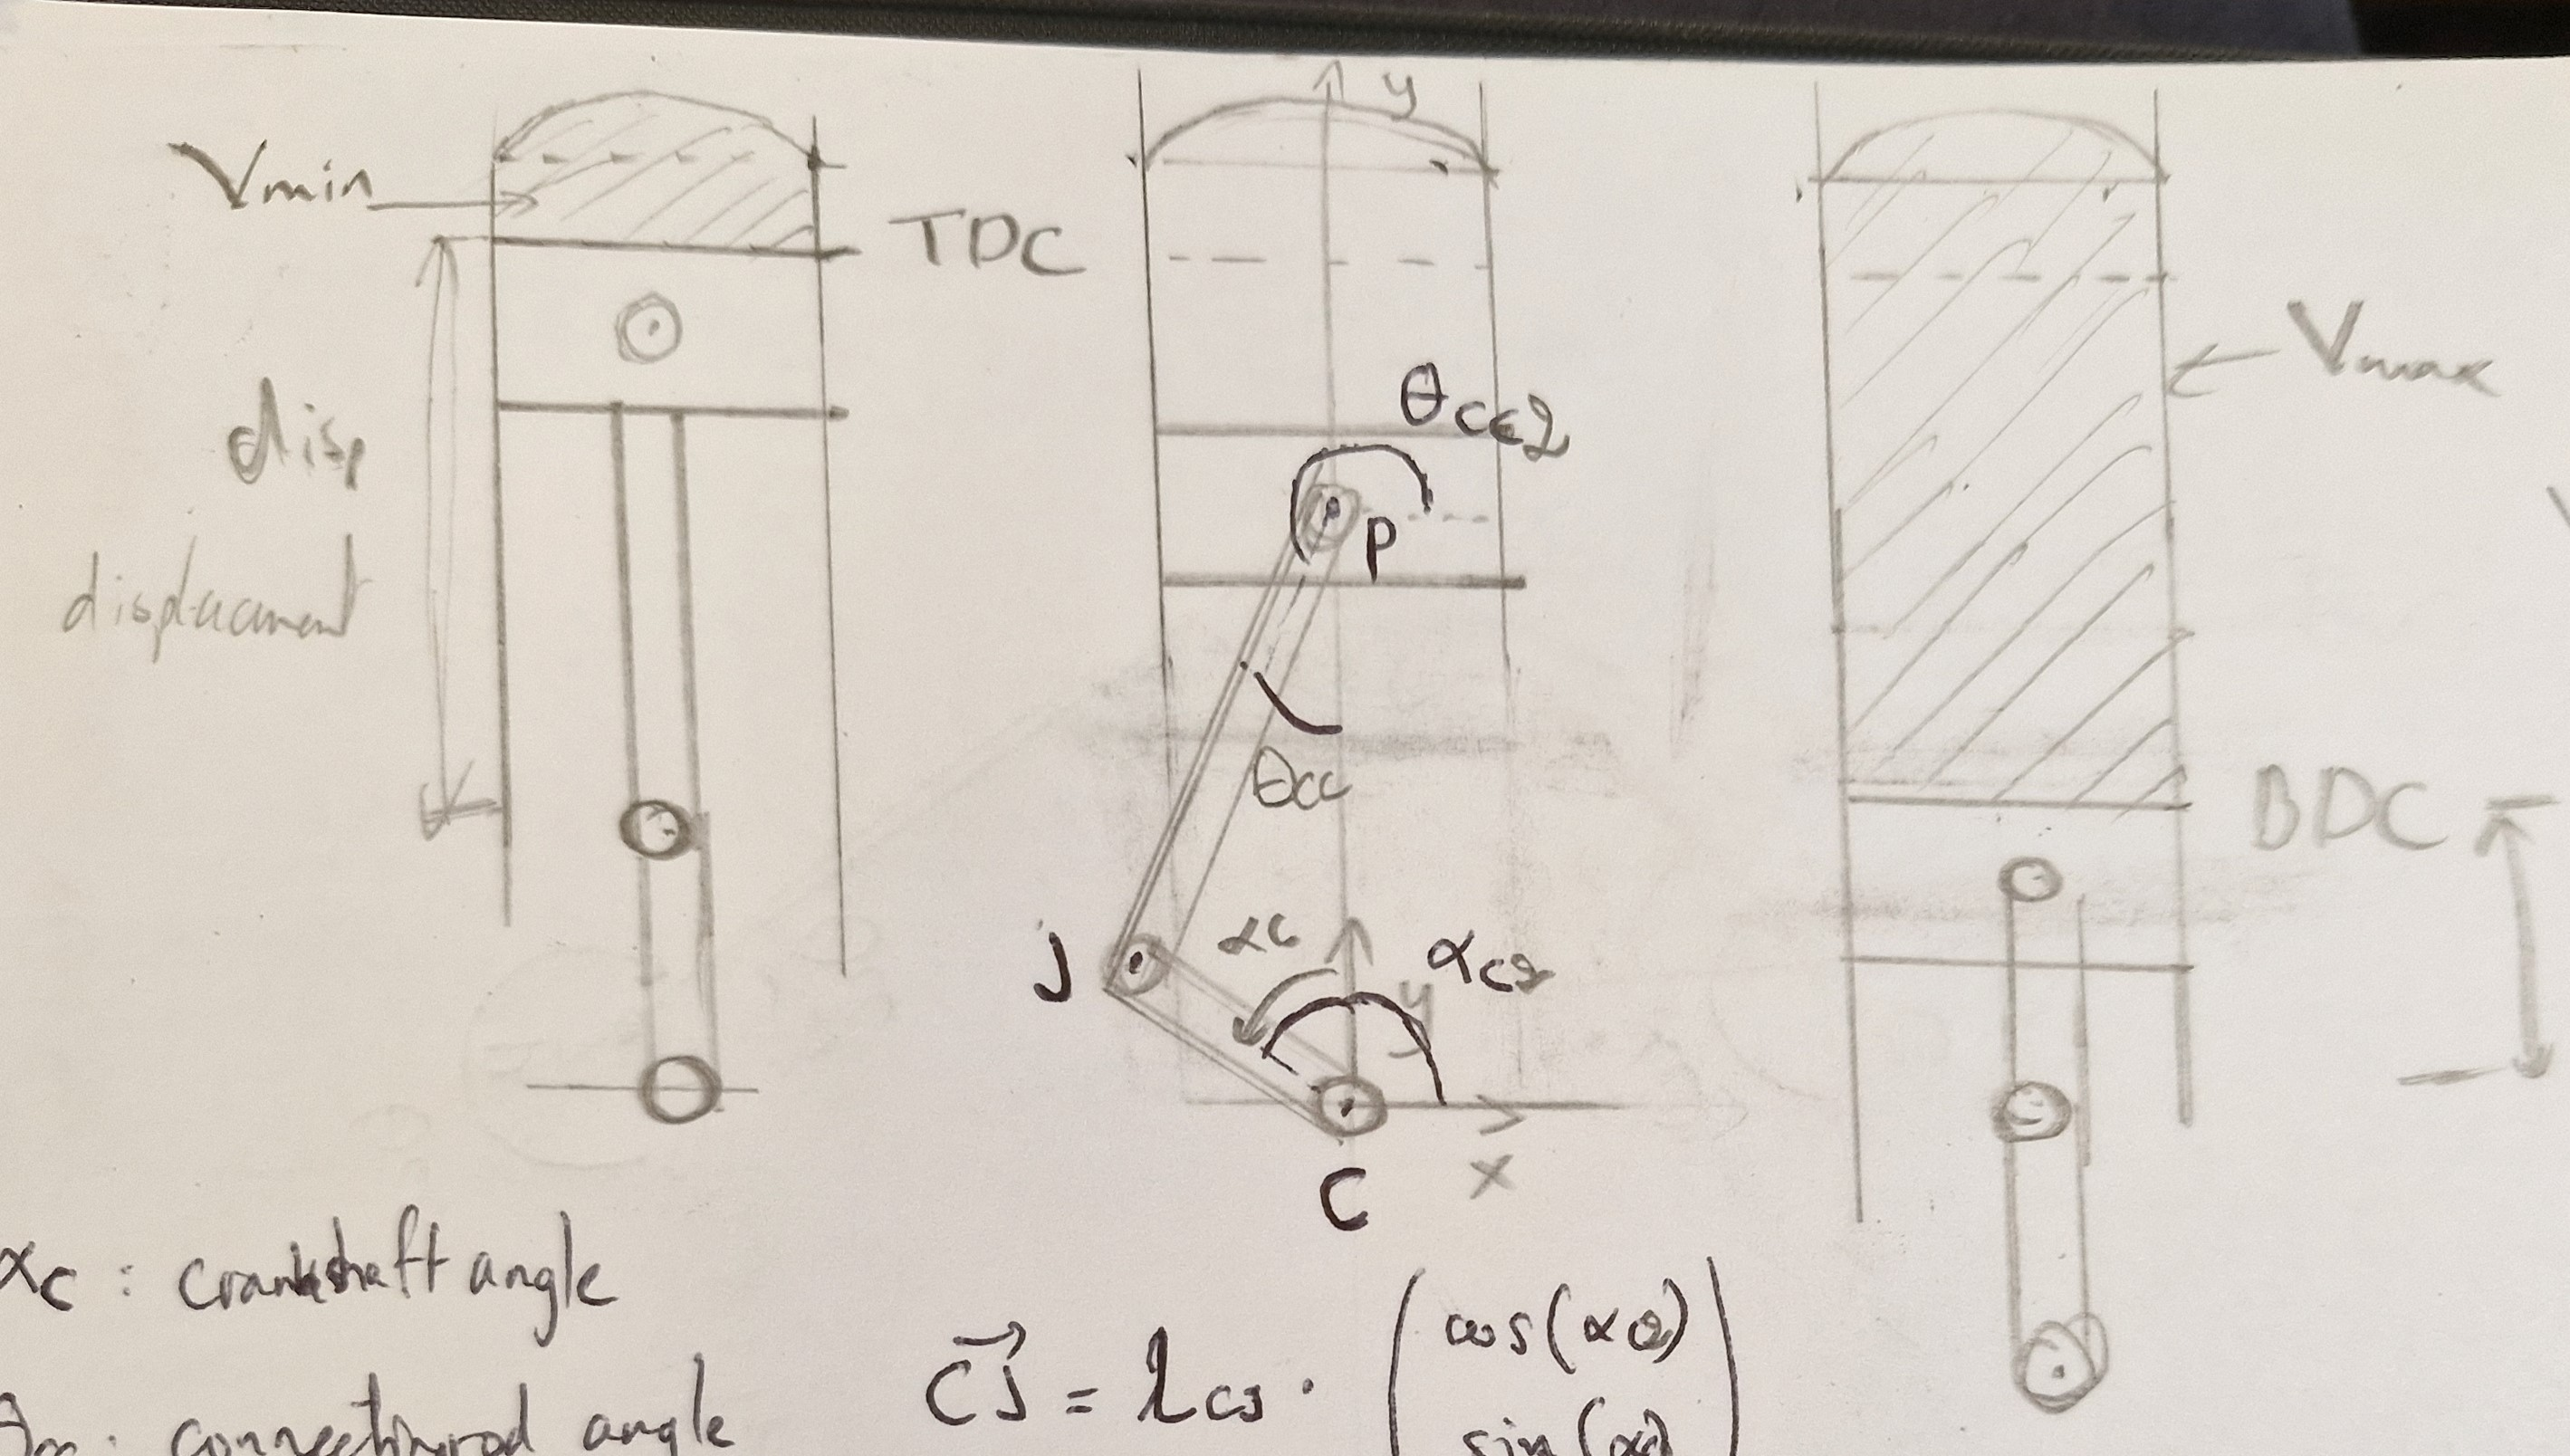
\includegraphics[scale=.2]{Engine_schema.jpg}
	
	main Referential, centered on the crankshaft :\\
	
	\begin{itemize}
		\item $x$ to the right
		\item y to the top
		\item z perpendicular to the plan formed by x and y .
		\item The piston head is moving in the $y$ direction.
	\end{itemize}
	
	we define angles by taking X-axis as reference
	
	Let's define the angle and position vector of each component
	

	1. Crankshaft
	\begin{eqnarray}
		\overline{CJ} = L_{CJ}\\
		\vec{CJ} = L_{CJ} \cdot 
		\begin{bmatrix}
			cos(\alpha_{c}) \\
			sin(\alpha_{c})\\
			0
		\end{bmatrix}_{R_{1}} \\
		\alpha_{c} \in [0, 2 \pi] 
	\end{eqnarray} 
	2. Connecting rod : 
	\begin{eqnarray}
		\overline{PJ} = L_{PJ}\\
		\vec{PJ} = L_{PJ} \cdot  
			\begin{bmatrix}
			cos(\theta_{cc}) \\
			sin(\theta_{cc}) \\
			0
		\end{bmatrix}_{R_{1}} \\
		\theta_{cc} \in [\theta_{cc}^{min}, \theta_{cc}^{max}]
	\end{eqnarray}
	3. Piston head: 
	\begin{eqnarray}
	\vec{CP} = L_{CP} \cdot  
	\begin{bmatrix}
		0 \\
		1 \\
		0
	\end{bmatrix}_{R_{1}} \\
	L_{CP} \text{ $\in$ } [BDC, TDC] = [BDC, BDC + disp]
	\end{eqnarray}
	\subsection{Newton-Raphson}
	The Newton-Raphson method is used to find the angle of the connecting rod. The following system of two equations must be solved : 
	\begin{eqnarray}
		\vec{CP} + \vec{PJ} + \vec{JC} = 0\\
		\vec{CP} + \vec{PJ} - \vec{CJ} = 0
	\end{eqnarray} 
	The two unknown variables are : 
	\begin{itemize}
		\item angle of the connecting rod : $\theta_{cc}$
		\item position of the piston head : $L_{CP}$
	\end{itemize}
	The driving variable is the crankshaft angle $\alpha_c$.
	For each value of this angle (from 0 to 360), the iteration of the Newton-Raphson method are executed until the system is solved. 
	The result will be the value of the unknown variables as function of the crankshaft angle. 
		
	with this we can define the range $[\theta_{cc}^{min}, \theta_{cc}^{max}]$ 
	\subsection{Thrust force}

		\item Establish the thrust force, along the $y$-axis $R_{1}$ : 
	During the combustion stroke, the burned air-fuel mixture pushed the piston head int the negative direction of the Y-axis.
	\begin{gather*}
		F_{thrust}=p \cdot S_{p}=p \cdot \pi \cdot\left(\frac{D}{2}\right)^{2}  \tag{2}\\
		\vec{F}_{\text {piston }}=\left[\begin{array}{c}
			0 \\
			- F_{thrust} \\
			0
		\end{array}\right]_{R_{1}} \tag{3}
	\end{gather*}
	
	
	$F_{\text {thrust }}$ : thrust force $[N]$\\
	$p$ : pressure inside the combustion chamber $[P a]$\\
	$D:$ piston diameter, bore $[m]$\\
	$S_{p}:$ piston head section $\left[m^{2}\right]$\\
	


		\item the thrust fore in the connecting rod referential is computed by rotating the previous vector with a rotation matrix . 
		the angle is the connecting rod angle $\theta_{cc}$, found using the results of the previous section, 
	\[
	\vec{F}_{thrust}^{R_{c c}}=F_{thrust} \cdot\left[\begin{array}{c}
		\cos \left(\theta_{c c}\right)  \tag{5}\\
		\sin \left(\theta_{c c}\right) \\
		0
	\end{array}\right]_{R_{c c}}
	\]
	
	$\theta_{c c}$ : angle between connecting rod and the $y$ axis\\
	
		
		Here, we can also add the energy consumed by the running gears : water pump, oil pump, alternator,\\
		
		\item Torque is the vector product of this force with the position of the crankin journal of the crankshaft,  from the center of the crankshaft. It should be oriented in the Z-direction.
		
		\[
		\vec{T}_{\text {piston }}=\vec{F}_{\text {thrust }}^{\text {total }} \times \text { position }_{c c}=\vec{F}_{\text {thrust }}^{\text {total }} \times\left[\begin{array}{c}
			\cos \left(\alpha_{c c}\right)  \tag{7}\\
			\sin \left(\alpha_{c c}\right) \\
			0
		\end{array}\right]_{R_{1}}
		\]
		
		$\alpha_{c c}$ : connecting rod angle according to $R_{1}$\\
		
		\item Power output is the scalar product of the torque with crankshaft angular speed
		
		
		\begin{equation*}
			\text { Power }=\vec{T}_{\text {piston }} \cdot \vec{\omega}_{engine} \tag{8}
		\end{equation*}
		
		\item Engine mechanical efficiency: quotient of output power by the input heat power (fuel power)
		
		\begin{equation*}
			\eta_{m}=\frac{\text { Power }}{\dot{Q}_{\text {in }}} \tag{9}
		\end{equation*}
		\item link cycle phases with 4 strokes with crankshaft angle
		then follow steps defined in Notion
		
	
	\end{enumerate}
	\subsection{Friction and consumption}
	The friction between The moving parts lead to power loss. 
	There are several ways to describe these loses 
	\begin{itemize}
		\item percentage of the total energy/power
		\item a friction coefficient to an existing force
		\item efficiency $\eta$ lower than 100$\%$
	\end{itemize}
	
	Here a non-exhaustive list of possible energy loses in ICE:
	\begin{itemize}
		\item mechanical loses : friction between moving part, between a part and a fluid (oil, water, ...)
		\item energy loses during combustion of the air- fuel mixture
		\item Piston friction : cylinder, piston pin,
		friction between piston head and cylinder:
	\begin{equation*}
		F_{\text {thrust }_{2}}=F_{thrust }-F_{fpcy} \tag{4}
	\end{equation*}
		\item Crankshaft friction : oil, bearing, connecting rod.
		
		power/energy lost because of between the crankshaft and oil
		\begin{equation*}
			\vec{F}_{thrust}^{total}=\vec{F}_{thrust}^{R_{c c}}+\vec{F}_{\text{oil friction }} \tag{6}
		\end{equation*}
		\item Water pump, oil pump, .... clutch, gearbox loses, transmission loses until reaching the wheels
	\end{itemize}
	these will reduce the overall efficiency of the engine.
	
	
	
	
	
	\[
	\overrightarrow{B C}_{R_{1}}=\left[\begin{array}{c}
		\overline{B C}_{x_{1}}  \tag{10}\\
		\overline{B C}_{y_{1}} \\
		0
	\end{array}\right]_{R_{1}}
	\]
	
	
	2. link cycle phases with 4 strokes with crankshaft angle. 

	
	\begin{equation}
		\vec{BC}_{R_{1}}=
		\begin{bmatrix}
			\overline{BC}_{x_1} \\
			\overline{BC}_{y_1}\\
			0
		\end{bmatrix}_{R_{1}} 
	\end{equation}
	
	\subsection{Engine thrust}
	Theorem of the preservation of linear momentum:
	\begin{equation}
		\int \int_{\Sigma} [P \cdot \vec{n}+ \rho \cdot \vec{V} (\vec{V} \cdot \vec{n})] = 0
	\end{equation}
	The term $\vec{V} \cdot \vec{n}$ is equal to zero when the velocity is perpendicular to the normal vector, which is the case on the lateral surface.
	What remain are the terms corresponding to the surfaces $A_0$ and $A_{10}$, which are perpendicular to the axis of the jet engine. 
	The thrust : 
	\begin{dmath}
		F = (P_{10} + \rho_{10} \cdot V_{10}^2) A_{10} - (P_{0} + \rho_{0} \cdot V_{0}^2) A_0 = P_{10} \cdot A_{10} + \rho_{10} \cdot V_{10}^2 \cdot A_{10} - P_{0} \cdot A_0 - \rho_{0} \cdot V_{0}^2 \cdot A_0
	\end{dmath}
	mass flow : 
	\begin{equation}
		\dot{m} = D = \rho \cdot V \cdot A
	\end{equation}
	
	\begin{dmath}
		F = P_{10} \cdot A_{10} + D_{10} \cdot V_{10} - P_{0} \cdot A_0 - D_{0} \cdot V_{0} = D_{10} \cdot V_{10} - D_{0} \cdot V_{0} + P_{10} \cdot A_{10} - P_{0} \cdot A_0
	\end{dmath}
	By using the simple trick of adding $P_0 \cdot A_{10} - P_0 \cdot A_{10}=0$
	
	\begin{dmath}
		F = D_{10} \cdot V_{10} - D_{0} \cdot V_{0} + P_{10} \cdot A_{10} - P_{0} \cdot A_0 + P_0 \cdot A_{10} - P_0 \cdot A_{10} = D_{10} \cdot V_{10} - D_{0} \cdot V_{0} + (P_{10} - P_0) A_{10} + P_0 (A_{10} -A_0)
	\end{dmath}
	
	It is useful to add the drag due to the engine housing: 
	\begin{equation}
		X_c = - \int \int P_c \cdot dA \vec{n} \vec{x} -> X_c = P_c (A_{10} - A_0)
	\end{equation}
	Where the $P_c$ is the pressure at the surface of the housing. 
	Historically, the first jet fighter, the Me-262, was equipped with two Junkers Jumo 004 B turbine engines with housings. So, these housings will produce each a drag force. 
	Since then, engines were housed inside the body of the jet fighter. In this case, this term is equal to 0. 
		
	Consequently, the thrust generated by an engine is : 
	
	\begin{dmath}
		F = D_{10} \cdot V_{10} - D_{0} \cdot V_{0} + (P_{10} - P_0) A_{10} + P_0 (A_{10} -A_0) -  P_c (A_{10} - A_0)
	\end{dmath}
	
	The pure engine thrust is : 
	\begin{dmath}
		F_{engine} = D_{10} \cdot V_{10} - D_{0} \cdot V_{0} + (P_{10} - P_0) A_{10}
	\end{dmath}
	Thrust due to the external fluid:  
	\begin{dmath}
		F_{fluid} = P_0 (A_{10} -A_0)
	\end{dmath}
	
	If the exhaust is adapted, then $P_{10} = P_0$, meaning that all the energy compressed in the engine will be converted to kinetic energy at the exhaust, in order to maximize the thrust. This is done thought modifiable nozzle to accommodate all working conditions. Depending on the measurements at the turbine (pressure, temperature, gas speed), the engine will modify the nozzle (section $A_{10}$ and shape) accordingly. 
	
	To make the plane harder to detect from heat-seeking missiles, the nozzle must be designed in order to reduce the Temperature of the gases at the exit as much as possible. 
	
	The plane manufacturer chooses the thrust needed to ensure that the plane has the specified performances, taking into account the drag due to the body shape of the plane. He also indicated the maximum volume that the engine can occupy in the plane.
	The engine manufacturer will design the engine to ensure to reach the specified thrust and air speed at the exit of the nozzle. The engine must fit into the volume specified by the plane manufacturer. 
	
	Naturally, other specifications must be fulfilled, like :
	\begin{itemize}
		\item low fuel consumption
		\item 
	\end{itemize}
	
	\newpage
	
	\section{Reminder}
	\subsection{Gases}
	\begin{eqnarray}
		P \cdot v= r \cdot T\\
		P \cdot V= m \cdot r \cdot T\\
		P \cdot V= n \cdot R \cdot T\\
		r = \frac{R}{M} = \frac{r}{m}\\
		W =\int P dV
	\end{eqnarray}
	V : volume [$m^3$] \\
	v : volume density [$\frac{m^3}{kg}$]
	
	\begin{eqnarray}
		P \cdot V^{\gamma} = const\\
		P_{in} \cdot (V_{in})^{\gamma} = P_{out} \cdot (V_{out})^{\gamma}\\
		W =\int P dV
	\end{eqnarray}
	
	\section{Engine computation}
	\begin{enumerate}
		\item Combustion chamber
		\item Turbine
		\item Compressor
		\item Inlet
		\item Nozzle
	\end{enumerate}

	
		 
	\newpage
	\begin{equation}
		\sum T_B = I_{BCE} \cdot \alpha
	\end{equation}
	$\sum T_B$ : total torques applied on point $B$ in [Nm]\\
	$I_{BCE}$ : inertia of the bucket in $[kg m^2]$\\
	$\alpha$: angular acceleration in $[\frac{rad}{s^2}] $
	
	The sum of torques in point $B$ can be expressed as the vector/cross product of force verctor and position vertor. 
	\begin{equation}
		\sum \vec{T_B} = \sum \vec{F} \times \vec{d}
	\end{equation}
	The result is a vector that is perpendicular to both vectors : 
	$\vec{T_B} \perp \sum \vec{F}$ and 
	$\vec{T_B} \perp \vec{d}$.
	
	Let's assume that $F_3$ is the sum of the torques applied on the triangle $BCE$. In this case, the application point of $F_3$ is $C$. The scalar value of $\vec{T_B}$ is  the segment $\overline{BC}$ multiplied by the tangential force. This one is the projection of $F_3$ on $x_2$ axis, $F_3^{x_2}$:
	\begin{equation}
		T_B=||\vec{T_B}|| = F_3^{x_2} \cdot \overline{BC}
	\end{equation}
	The projection of $F_3$ on $x_2$ axis, $F_3^{y_2}$ is $\parallel$ to the segment $BC$. In this case, the vector/cross product is equal to $0$.
	Or : 
	\begin{equation}
		T_B=||\vec{T_B}|| = F_3 \cdot \overline{BF}
	\end{equation}
	% 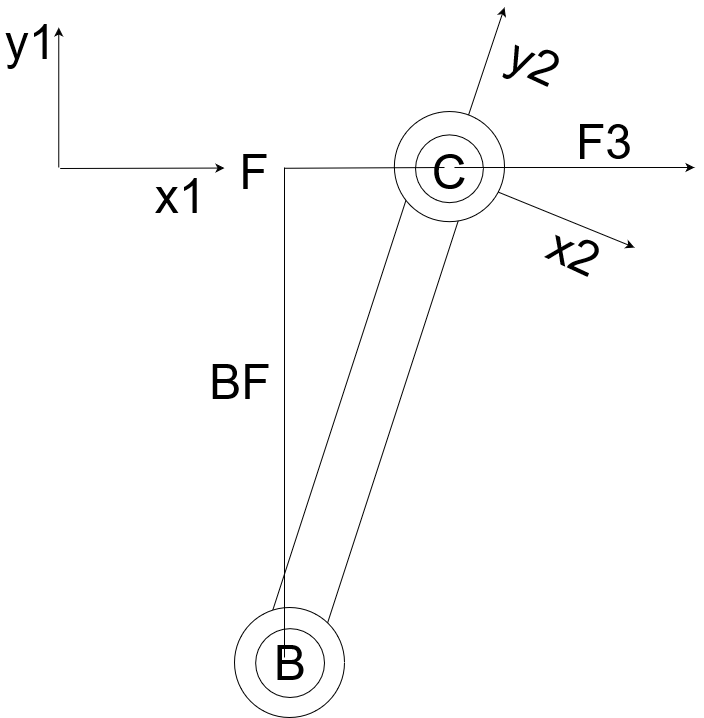
\includegraphics[scale=.35]{BCF.drawio.png}
	
	$\overline{B F}$ is the shortest distance between the force $F_3$ and point $B$.
	$\overline{B F}$ : projection of segment $\overline{BC}$ on axis $y_1$. 
	
	\begin{equation}
		\vec{BC}_{R_{1}}=
		\begin{bmatrix}
			\overline{BC}_{x_1} \\
			\overline{BC}_{y_1}\\
			0
		\end{bmatrix}_{R_{1}} 
	\end{equation}
	or : $F_3$ multiplied by $AD$, the distance between $F_3$ and $B$. (add schema with this 2 examples)
	
	Generally speaking, sum of Torque in B is 
	1. the sum of tangantial forces multiplied by
	2. easier : vector/cross product of a vector and distance vector to the $B$ point.  
	
	The Reynolds number is an non-dimensional number, and used to define if the fluid flow is laminar or turbulent. 
	
	\begin{equation}
		Re = \frac{\rho \cdot u \cdot L}{\mu}
	\end{equation}
	$\rho$ : density of the fluid\\
	$u$ : flow speed\\
	$L$ : characteristic linear dimension\\
	$\mu$ : dynamic viscosity of the fluid\\
	
	The characteristic linear dimension $L$ depends on the shape of the object of study. Here some example : 
	\begin{itemize}
		\item Plane wing : length of the wing
		\item Hydraulic pipe : diameter of the pipe
		\item Complex shape : the biggest dimension
	\end{itemize}
	Depending of the result, the flow can have 3 regimes
	
	\begin{itemize}
		\item If $Re$ <~ 2040, the flow is still considered laminar 
		\item If $Re$ >~ 2100, the flow is turbulent
		\item If 1800 <~ $Re$ <~ 2100, the flow is in the transition/intermediary range, which is a mix of laminar and turbulent \footnote{\url{https://en.wikipedia.org/wiki/Laminar_flow}}
	\end{itemize}
	
	For each regime, the drag force is different. 
	For turbulent and laminar regimes, the formula is as follows:
	\begin{equation}
		F_d^{turbulent} = \frac{1}{2} \cdot \rho \cdot C_D \cdot S \cdot u^2
	\end{equation}
	
	\begin{equation}
		F_d^{laminar} = C_F \cdot \rho \cdot  D^2 \cdot u^2\\
	\end{equation}
	$S$: cross frontal section\\
	$C_D$ : turbulent drag coefficient\\
	$C_F$ : laminar drag coefficient\\
	
	The intermediary regime is a mix from the 2 base regimes. In this situation, an approximation can be evaluated by computed the percent $Re$ compared to 1800 and 2100. 
	\begin{equation}
		F_d^{transition} = (1- \frac{Re - 1800}{2100-1800}) \cdot F_d^{laminar} + \frac{Re - 1800}{2100-1800} \cdot F_d^{turbulent}
	\end{equation}
	
	
	\newpage
	\section{Techniques}
	Prefabricated parts (PFP) /pre-manufactured parts (PMP)
	
	Instead of creating the same parts again and again, design the components and make them easily modifiable.
	for example, combine 2 parts to create a third one, which is useful in an other application. Then add them to the system in the assembly
	Example : threads : try the smallest possible size, for example M3 to M20. 
	
	Test them with small parts and check the tolerances. 
	The next step is to prepare small parts ready to be added to system parts. The final step is the merge the bodies. 
	
	
	table
	
	\begin{table}[ht]
		\caption{Holes and threaded holes} % title of Table
		\centering % used for centering table
		\begin{tabular}{c c c} % centered columns (4 columns)
			\hline\hline %inserts double horizontal lines
			Screw & Threaded hole diameter & Bore Hole (clearance) \\ [0.5ex] % inserts table
			%heading
			\hline % inserts single horizontal line
			M3 & 2.8 & 3.2 \\ % inserting body of the table
			4 & 35 & 144 \\
			5 & 45 & 300 \\ [1ex] % [1ex] adds vertical space
			\hline %inserts single line
		\end{tabular}\label{table:nonlin} % is used to refer this table in the text
	\end{table}
	
	Clearance
	To fix two part together, a clearance is needed.
	When two parts must be assembled together, a clearance of 0.1mm is enough. Then use the glue to fix the assembly. 
	
	
	
	\begin{table}[ht]
		\caption{Nonlinear Model Results} % title of Table
		\centering % used for centering table
		\begin{tabular}{c c c c} % centered columns (4 columns)
			\hline\hline %inserts double horizontal lines
			Case & Method\#1 & Method\#2 & Method\#3 \\ [0.5ex] % inserts table
			%heading
			\hline % inserts single horizontal line
			1 & 50 & 837 & 970 \\ % inserting body of the table
			2 & 47 & 877 & 230 \\
			3 & 31 & 25 & 415 \\
			4 & 35 & 144 & 2356 \\
			5 & 45 & 300 & 556 \\ [1ex] % [1ex] adds vertical space
			\hline %inserts single line
		\end{tabular}\label{table:nonlin} % is used to refer this table in the text
	\end{table}
	
	
	
	\begin{equation}
		Length_{lattitude}(\phi) = 111132.92-559.82 \cdot cos(2 \cdot \phi)+1.175*cos(4 \cdot \phi)-0.0023 \cdot cos(6 \cdot \phi)= ... [m/degree]
	\end{equation}
	1 degree longitude at latitude phi
	\begin{equation}
		Length_{longitude}(\phi) =
		111412.84-93.5 \cdot cos(3 \cdot \phi)+ 0.118 \cdot cos(5 \cdot \phi)= ... [m/degree]
	\end{equation}
	
	\newpage
	\section{Schéma cinématique}
	
	
	\subsection{Vecteurs positions}
	origine : centre de rotation verticale se trouvant sous les pâles principales.
	\medbreak
	position  des pâles principales ($pp$) : vecteur verticale
	\medbreak
	position de l'hélice arrière : 
	vecteur allant de l'origine vers l'hélice ($h$) arrière. 
	
	
	\newpage
	\section{Angular momentum}
	
	\subsection{Formula}
	\begin{equation}
		\vec{L}=\vec{OA} \otimes \vec{P}=\vec{r} \otimes \vec{P}=\vec{r} \otimes m \cdot \vec{v}=\vec{I} \otimes \vec{\omega}
	\end{equation}
	$\vec{L}$ : Angular Momentum [$kg \cdot \frac{m^2}{s}$]\\
	$\vec{OA}$ and $r$: position of the mass [$m$] according to a referance\\
	$\vec{P}$ : linear momentum [$kg\cdot \frac{m}{s}$]\footnote{$\vec{L}$ is perpendicular to both $\vec{P}$ and $\vec{r}$}\\
	$\vec{v}$ : velocity [$\frac{m}{s}$]
	$I$ : moment of inertia [$m^2 \cdot kg \cdot$]\\
	$\omega$ : angular speed [$\frac{rad}{s}$]
	
	Torque : 
	\begin{equation}
		M = \frac{d\vec{L}}{dt}=\frac{d(\vec{I} \otimes \vec{\omega})}{dt}
	\end{equation}
	\medbreak
	if we consider a particule of mass $m$, $\vec{r}$ is the position of the center of mass.
	If it is a solid object, $L$ is first computed according to the axis of rotation of the object : 
	\begin{equation}
		\vec{L}_{ar}=\vec{I}_{ar} \otimes \vec{\omega}_{ar}
	\end{equation}
	To compute the angular moment according to an other axis of rotation (new referance), we use the Huygens-Steiner theorem (or the Parallel axis theorem) : 
	\begin{equation}
		\vec{L}_{0}=\vec{I}_{0} \otimes \vec{\omega}_{cm}\\
	\end{equation}
	\begin{equation}
		\vec{I}_{0} = \vec{I}_{ar} + m\cdot d^2
	\end{equation}
	with $d$ the distance between the axis of rotation of the object and the new referance. 
	\subsection{Condition of stability}
	
	Main rotor(s):
	\begin{equation}
		\vec{L}_{mr}=\vec{r}_{mr} \otimes m_{mr} \cdot \vec{v_{mr}}=\vec{I_{mr}} \otimes \vec{\omega_{mr}}
	\end{equation}
	
	
	Rear rotor : 
	\begin{equation}
		\vec{L}_{rr}=\vec{r}_{rr} \otimes m_{rr} \cdot \vec{v_{rr}}=\vec{I_rr} \otimes \vec{\omega_{rr}}
	\end{equation}
	
	assurer la stabilité lors du vol: les moments cinétiques doivent s'annuler. (poser la formule et résoudre)
	\begin{equation}
		\vec{L_{mr}}=\vec{L_{rr}}
	\end{equation}
	
	or
	
	The generated torque is compensated : 
	\begin{equation}
		\sum \vec{M_{mr}}=\sum \vec{M_{rr}}
	\end{equation}
	
	find a relation between $\omega_{mr}$ and $\omega_{rr}$ -> determine the transmission ratio
	
	\subsection{Pivots à droite et à gauche}
	pour tourner à gauche ou doite, on ne doit plus satisfaire la condition de stabilité. le pilote utiliser le pédalier pour accélérer/ralentir l'hélice arrière. ainsi les moments cinétiques ne sont plus égaux.
	\medbreak
	calculer l'effet de rotation sur l'hélicoptère si l'hélice est accélérée/ralentie de 10,20,30,.. $\%$. mettre un tableau. calculer la vitesse de rotation dans ces cas-là. 
	
	
	\begin{equation}
		\begin{bmatrix}
			0 \\
			0\\
			l_1
		\end{bmatrix}_{R_{1}} \enspace
		\vec{AB}_{R_{2}}=
		\begin{bmatrix}
			0 \\
			l_2\\
			0
		\end{bmatrix}_{R_{2}} \enspace
		\vec{BC}_{R_{3}}=
		\begin{bmatrix}
			l_3 \\
			0\\
			0
		\end{bmatrix}_{R_{3}} \enspace
		\vec{CD}_{R_{4}}=
		\begin{bmatrix}
			0 \\
			0\\
			-l_4
		\end{bmatrix}_{R_{4}} \enspace
	\end{equation}
	
	\begin{itemize}
		\item
		\item 
		\item 
	\end{itemize}
	
	
	\medbreak
	
	\medbreak
	
	\medbreak
	
	\medbreak
	
	
	
	
	\begin{equation}
		\begin{split}
			\vec{OE}_R=\vec{OA}_R+\vec{AB}_R+\vec{B B_1}_R+\vec{B_1 C_1}_R+\vec{C_1 C}_R\\+\vec{C C_2}_R+\vec{C_2 D}_R+\vec{D D_1}_R+\vec{D_1 E}_R
		\end{split}
	\end{equation}
	
	\begin{equation}
		\begin{split}
			\vec{OF}_R=\vec{OA}_R+\vec{AB}_R+\vec{B B_1}_R+\vec{B_1 C_1}_R+\vec{C_1 C}_R\\+\vec{C C_2}_R+\vec{C_2 D}_R+\vec{D D_1}_R+\vec{D_1 E}_R+\vec{E F}_R
		\end{split}
	\end{equation}
	
	\begin{equation}
		\begin{split}
			\vec{OG}_R=\vec{OA}_R+\vec{AB}_R+\vec{B B_1}_R+\vec{B_1 C_1}_R+\vec{C_1 C}_R+\vec{C C_2}_R\\+\vec{C_2 D}_R+\vec{D D_1}_R+\vec{D_1 E}_R+\vec{E F}_R+\vec{F F_3}_R+\vec{F_3 G}_R
		\end{split}
	\end{equation}
	
	\begin{equation}
		\begin{split}
			\vec{OH}_R=\vec{OA}_R+\vec{AB}_R+\vec{B B_1}_R+\vec{B_1 C_1}_R+\vec{C_1 C}_R+\vec{C C_2}_R+\vec{C_2 D}_R\\+\vec{D D_1}_R+\vec{D_1 E}_R+\vec{E F}_R+\vec{F F_3}_R+\vec{F_3 G}_R+\vec{G H}_R
		\end{split}
	\end{equation}
	
	
	\section{Conclusion}
	
	
\end{document}